\chapter{Lehrveranstaltungen}
\label{lehrveranstaltung}
Als Lehrveranstaltung wird im Gesamtsystem das gleiche verstanden, wie im Antrag des Studiengangs. Die Lehrveranstaltung wird immer aus Sicht eines Studiengangs oder aus der Sicht des Studenten gesehen. Der Titel der Lehrveranstaltung findet sich im Zeugnis und im Lehre-Bereich im CIS wieder. Nicht zu verwechseln ist die Lehrveranstaltung mit dem Lehrfach oder der Lehreinheit (siehe eigene Kapiteln).\\
Einmal verwendete Lehrveranstaltungen k�nnen nicht mehr entfernt sondern nur deaktiviert werden, da Notenzuordnungen verloren gehen w�rden.
\section{Aufbau} 
Folgende Attribute bestimmen eine Lehrveranstaltung:
\begin{table*}[htbp]
	\centering
		\begin{tabular}{|r|l|}
			\hline
			Kuerzel & Abk�rzung der LV. Mindestens 2, maximal 5 Zeichen. \\&3,4 od. 5tes Zeichen darf eine Ziffer sein.\\& Buchstaben sollten einheitlich gro� geschrieben werden.\\
			\hline
			Bezeichnung & Name der Lehrveranstaltung (max. 64 Zeichen)\\
			\hline
			LehreVz	& Der Name des Lehreverzeichnisses sollte mit dem K�rzel �bereinstimmen. 
				\\&Es sind ausschlie�lich kleingeschriebene Buchstaben zu verwenden. 
				\\&Dies legt fest, wie der Ordner der LV im Filesystem heisst. 
				\\&Wenn 2 Lehrveranstaltungen im selben Studiengang und Semester das gleiche 
				\\&Lehreverzeichnis eingetragen haben, dann wird im CIS f�r beide LVs das gleiche 
				\\&Download, Upload und Semesterplanverzeichnis verwendet.\\
			\hline
		\end{tabular}
	\caption{Attribute der Lehrveranstaltung}
	\label{tab:AttributeDerLehrveranstaltung}
\end{table*}
\section{Bearbeiten von LV-Eintr�gen}
Kommt es zu Curriculums�nderungen, stehen dem FAS-Anwender einige Anpassungsm�glichkeiten zur Verf�gung. Der Aufruf erfolgt durch Anklicken von Men�punkt \textit{Lehrveranstaltungsverwaltung} unter \textsl{Extras} wie Abbildung \ref{LV} zeigt.
\begin{figure}
	\centering
	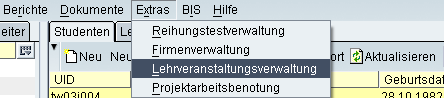
\includegraphics[width=0.75\textwidth]{FAS_LV.png}
	\caption{Bearbeiten von Lehrveranstaltungseintr�gen}
	\label{LV}
\end{figure}
Der Anwender gelangt daraufhin auf die in Abbildung \ref{LV1} gezeigte Seite in einem neuen Fenster. Zuerst werden in den Auswahlfeldern links oben, Studiengang und Semester ausgew�hlt. Zus�tzlich kann die Ausgabe auch noch auf einen Fachbereich eingeschr�nkt werden. Zum Aktualisieren der Anzeige wird dann noch die Taste \textit{Anzeigen} angeklickt. Es werden alle \emph{aktiven} Lehrveranstaltungen, die den angegebenen Kriterien entsprechen, angezeigt. Es k�nnen folgende Werte ver�ndert werden:
\begin{enumerate}
	\item Lehre: Wenn angehakt, erscheint die LV auf der CIS-Seite.
	\item Sort: Die eingegebenen Zahlen bestimmen die Reihenfolge der LVs auf dem Semesterzeugnis.
	\item Incoming: Legt die Anzahl an Incoming fest, die an dieser Lehrveranstaltung teilnehmen d�rfen.
	\item Zeugnis: Wenn angehakt, erscheint die LV auf den Zeugnisausdrucken und Studienerfolgsbest�tigungen.
	\item BA/DA: Wenn angehakt, k�nnen Projektarbeiten zugeordnet werden.
	\item FBK: Hier kann ein Koordinator f�r diese LV ausgew�hlt werden. Dieses Feld mu� nur bef�llt werden, wenn der verantwortliche Koordinator nicht
	 mit dem Fachbereichskoordinator �bereinstimmt. Bleibt das Feld leer, wird der Fachbereichskoordinator zugeordnet. In dem DropDown scheinen nur 			 
	 Personen auf, denen die Funktion Koordinator f�r diesen Studiengang/Institut zugeordnet ist.
	\item LVInfo: Hier k�nnen die LVInfos von einer anderen Lehrveranstaltung kopiert werden. Dazu muss in das Feld die ID der Lehrveranstaltung eingetragen werden, von der die LVInfo kopiert werden soll. LVInfos k�nnen nur dann kopiert werden, wenn noch keine LVInfo angelegt ist.
\end{enumerate}
Bei den Feldern Lehre, Zeugnis und BA/DA ist nur ein einfacher Klick und kein Doppelklick zur Zustands�nderung notwendig. Die Eingabe in Textfelder wird mit einem Klick auf die Taste \textit{ok} am rechten Feldrand gespeichert. Mit dem Schlie�en des Fensters wird die Bearbeitung der Lehrveranstaltungen beendet.
\begin{figure}
	\begin{center}
    \begin{picture}(155,45)
			\put(0,0){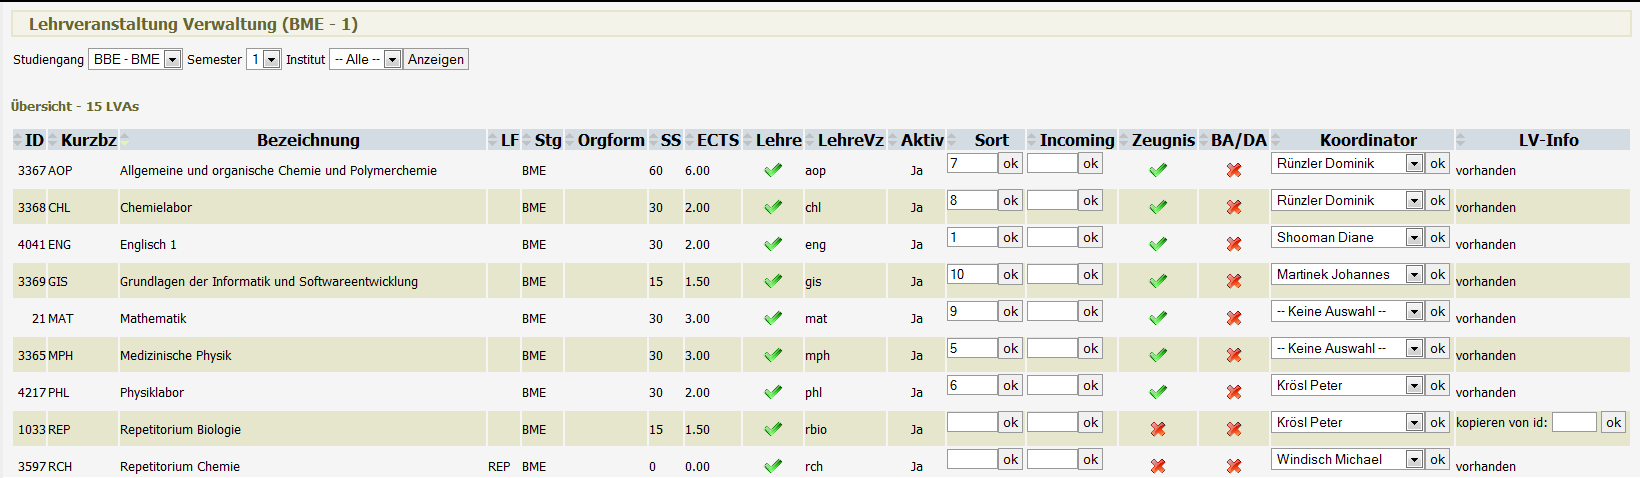
\includegraphics[height=70mm, width=155mm]{FAS_LV1.png}}
			\markier{1}{72}{61}{1}{-1}
			\markier{2}{86}{61}{1}{-1}
			\markier{2}{93}{61}{1}{-1}
			\markier{3}{100}{61}{1}{-1}
			\markier{4}{107}{61}{1}{-1}
			\markier{5}{120}{61}{1}{-1}
			\markier{6}{134}{61}{1}{-1}
		\end{picture}
    \caption{Lehrveranstaltungen}
		\label{LV1}
  \end{center}
\end{figure}
